\chapter{Virtauslaskenta}

Lähtökohtanamme on suunnattu verkko, jossa on kaksi erityistä solmua:
\emph{lähtösolmu} ja \emph{kohdesolmu}.
Jokaisella kaarella on paino, joka rajoittaa,
miten paljon virtausta voi kulkea kaarta pitkin,
ja haluamme selvittää, mikä on \emph{maksimivirtaus} lähtösolmusta
kohdesolmuun.

Lähtökohtanamme on suunnattu verkko, jossa on kaksi erityistä solmua:
\emph{lähtösolmu} ja \emph{kohdesolmu}.
Jokaisella kaarella on paino, joka rajoittaa,
miten paljon virtausta voi kulkea kaarta pitkin,
ja haluamme selvittää, mikä on \emph{maksimivirtaus} lähtösolmusta
kohdesolmuun.

\section{Maksimivirtaus}

Maksimivirtausongelmassa haluamme selvittää
suurimman \emph{virtauksen} suunnatun verkon
lähtösolmusta kohdesolmuun.
Virtaus lähtee liikkeelle lähtö\-solmusta ja saapuu kohdesolmuun
niin, että jokaiseen välisolmuun tuleva virtaus on
yhtä suuri kuin solmusta lähtevä virtaus.
Jokaisella kaarella on \emph{kapasiteetti}, jota virtauksen
määrä kaarta pitkin ei saa ylittää.

\begin{figure}
\center
\begin{center}
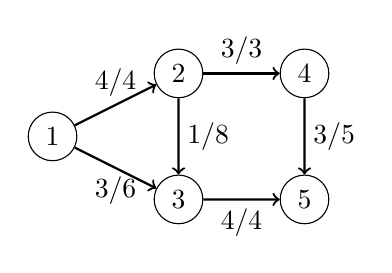
\begin{tikzpicture}[scale=0.8,label distance=-1.5mm]
\node[draw, circle] (1) at (0,-1) {$1$};
\node[draw, circle] (2) at (2,0) {$2$};
\node[draw, circle] (3) at (2,-2) {$3$};
\node[draw, circle] (4) at (4,0) {$4$};
\node[draw, circle] (5) at (4,-2) {$5$};
\path[draw,thick,->] (1) -- node[font=\small,label=above:$4/4$] {} (2);
\path[draw,thick,->] (1) -- node[font=\small,label=below:$3/6$] {} (3);
\path[draw,thick,->] (2) -- node[font=\small,label=right:$1/8$] {} (3);
\path[draw,thick,->] (2) -- node[font=\small,label=above:$3/3$] {} (4);
\path[draw,thick,->] (3) -- node[font=\small,label=below:$4/4$] {} (5);
\path[draw,thick,->] (4) -- node[font=\small,label=right:$3/5$] {} (5);
\end{tikzpicture}
\end{center}
\caption{Maksimivirtaus solmusta $1$ solmuun $5$ on $7$.}
\label{fig:makvir}
\end{figure}

Tarkastellaan esimerkkinä kuvan \ref{fig:makvir} verkkoa.
Tässä verkossa maksimivirtaus solmusta $1$ solmuun $5$ on $7$.
Jokaisessa kaaressa merkintä $v/k$ tarkoittaa,
että kaaren kautta kulkee virtausta $v$ ja
kaaren kapasiteetti on $k$.
Solmusta $1$ lähtevä virtauksen määrä on $4+3=7$,
solmuun $5$ saapuva virtauksen määrä on $3+4=7$
ja kaikissa muissa solmuissa saapuva virtaus
on yhtä suuri kuin lähtevä virtaus.

\subsection{Ford-Fulkersonin algoritmi}

Ford-Fulkersonin algoritmi on tunnetuin menetelmä verkon
maksimivirtauksen etsimiseen,
ja tutustumme seuraavaksi tämän algoritmin toimintaan.
Algoritmi etsii polkuja lähtösolmusta kohdesolmuun,
jotka kasvattavat virtausta pikkuhiljaa.
Kun mitään polkua ei voi enää muodostaa, algoritmi on onnistunut
muodostamaan maksimivirtauksen.

\begin{figure}
\center
\begin{center}
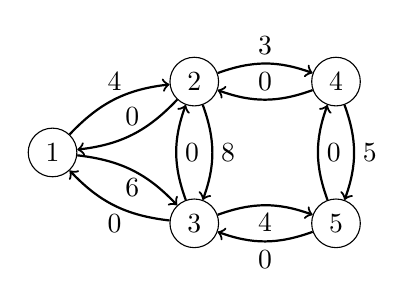
\begin{tikzpicture}[scale=0.9,label distance=-1.5mm]
\node[draw, circle] (1) at (0,-1) {$1$};
\node[draw, circle] (2) at (2,0) {$2$};
\node[draw, circle] (3) at (2,-2) {$3$};
\node[draw, circle] (4) at (4,0) {$4$};
\node[draw, circle] (5) at (4,-2) {$5$};
\path[draw,thick,->] (1) edge [bend left=20] node[font=\small,label=above:$4$] {} (2);
\path[draw,thick,->] (2) edge [bend left=20] node[font=\small,label=above:$0$] {} (1);
\path[draw,thick,->] (1) edge [bend left=20] node[font=\small,label=below:$6$] {} (3);
\path[draw,thick,->] (3) edge [bend left=20] node[font=\small,label=below:$0$] {} (1);
\path[draw,thick,->] (2) edge [bend left=20] node[font=\small,label=right:$8$] {} (3);
\path[draw,thick,->] (3) edge [bend left=20] node[font=\small,label=right:$0$] {} (2);
\path[draw,thick,->] (2) edge [bend left=20] node[font=\small,label=above:$3$] {} (4);
\path[draw,thick,->] (4) edge [bend left=20] node[font=\small,label=above:$0$] {} (2);
\path[draw,thick,->] (3) edge [bend left=20] node[font=\small,label=below:$4$] {} (5);
\path[draw,thick,->] (5) edge [bend left=20] node[font=\small,label=below:$0$] {} (3);
\path[draw,thick,->] (4) edge [bend left=20] node[font=\small,label=right:$5$] {} (5);
\path[draw,thick,->] (5) edge [bend left=20] node[font=\small,label=right:$0$] {} (4);
\end{tikzpicture}
\end{center}
\caption{Verkon esitysmuoto Ford-Fulkersonin algoritmissa.}
\label{fig:floesi}
\end{figure}

Algoritmin käyttäminen vaatii, että verkko on esitetty
erityisessä muodossa, jossa jokaista alkuperäisen verkon
kaarta vastaa kaksi kaarta:
alkuperäinen kaari, jonka painona on aluksi kaaren kapasiteetti,
sekä sille kään\-teinen kaari, jonka painona on aluksi $0$.
Käänteisten kaarten avulla pystymme tarvittaessa \emph{peruuttamaan}
virtausta algoritmin aikana.
Kuva \ref{fig:floesi} näyttää, kuinka esitämme esimerkkiverkkomme algoritmissa.

Algoritmin jokaisessa vaiheessa muodostamme polun
lähtösolmusta kohdesolmuun.
Polku voi olla mikä tahansa, kunhan jokaisen kaaren paino
polulla on positiivinen.
Polun muodostamisen jälkeen virtaus lähtösolmusta kohdesolmuun
kasvaa $p$:llä, missä $p$ on pienin kaaren paino polulla.
Lisäksi jokaisen polulla olevan kaaren paino vähenee $p$:llä
ja jokaisen niille käänteisen kaaren paino kasvaa $p$:llä.
Etsimme vastaavasti uusia polkuja, kunnes mitään sallittua
polkua ei voi enää muodostaa.

Kuva \ref{fig:floesi} näyttää, kuinka Ford-Fulkersonin algoritmi muodostaa
maksimivirtauksen esimerkkiverkossamme.
Algoritmi muodostaa ensin polun $1 \rightarrow 2 \rightarrow 3 \rightarrow 5$,
jossa pienin paino on $4$.
Tämän seurauksena virtaus kasvaa $4$:llä,
polulla olevien kaarten paino vähenee $4$:llä
ja käänteisten kaarten paino kasvaa $4$:llä.
Tämän jälkeen algoritmi muodostaa polun
$1 \rightarrow 3 \rightarrow 2 \rightarrow 4 \rightarrow 5$,
joka kasvattaa virtausta $3$:lla.
Huomaa, että tämä polku peruuttaa
kaarta $2 \rightarrow 3$ menevää virtausta,
koska se kulkee käänteisen kaaren $3 \rightarrow 2$ kautta.
Tämän jälkeen algoritmi ei enää pysty muodostamaan mitään polkua
solmusta $1$ solmuun $5$, joten maksimivirtaus on $4+3=7$.

\begin{figure}
\center
\begin{center}
\begin{tikzpicture}[scale=0.9,label distance=-1.5mm]
\newcommand\verkko[0]{
\node[draw, circle] (1) at (0,-1) {$1$};
\node[draw, circle] (2) at (2,0) {$2$};
\node[draw, circle] (3) at (2,-2) {$3$};
\node[draw, circle] (4) at (4,0) {$4$};
\node[draw, circle] (5) at (4,-2) {$5$};
}
\begin{scope}
\verkko
\path[draw,thick,->] (1) edge [bend left=20] node[font=\small,label=above:$4$] {} (2);
\path[draw,thick,->] (2) edge [bend left=20] node[font=\small,label=above:$0$] {} (1);
\path[draw,thick,->] (1) edge [bend left=20] node[font=\small,label=below:$6$] {} (3);
\path[draw,thick,->] (3) edge [bend left=20] node[font=\small,label=below:$0$] {} (1);
\path[draw,thick,->] (2) edge [bend left=20] node[font=\small,label=right:$8$] {} (3);
\path[draw,thick,->] (3) edge [bend left=20] node[font=\small,label=right:$0$] {} (2);
\path[draw,thick,->] (2) edge [bend left=20] node[font=\small,label=above:$3$] {} (4);
\path[draw,thick,->] (4) edge [bend left=20] node[font=\small,label=above:$0$] {} (2);
\path[draw,thick,->] (3) edge [bend left=20] node[font=\small,label=below:$4$] {} (5);
\path[draw,thick,->] (5) edge [bend left=20] node[font=\small,label=below:$0$] {} (3);
\path[draw,thick,->] (4) edge [bend left=20] node[font=\small,label=right:$5$] {} (5);
\path[draw,thick,->] (5) edge [bend left=20] node[font=\small,label=right:$0$] {} (4);
\path[draw,thick,->,red,line width=2pt] (1) edge [bend left=20] (2);
\path[draw,thick,->,red,line width=2pt] (2) edge [bend left=20] (3);
\path[draw,thick,->,red,line width=2pt] (3) edge [bend left=20] (5);
\draw[->,thick] (5.5,-1) -- (6.5,-1);
\node at (6,-3) {vaihe 1};
\end{scope}
\begin{scope}[xshift=7.5cm]
\verkko
\path[draw,thick,->] (1) edge [bend left=20] node[font=\small,label=above:$0$] {} (2);
\path[draw,thick,->] (2) edge [bend left=20] node[font=\small,label=above:$4$] {} (1);
\path[draw,thick,->] (1) edge [bend left=20] node[font=\small,label=below:$6$] {} (3);
\path[draw,thick,->] (3) edge [bend left=20] node[font=\small,label=below:$0$] {} (1);
\path[draw,thick,->] (2) edge [bend left=20] node[font=\small,label=right:$4$] {} (3);
\path[draw,thick,->] (3) edge [bend left=20] node[font=\small,label=right:$4$] {} (2);
\path[draw,thick,->] (2) edge [bend left=20] node[font=\small,label=above:$3$] {} (4);
\path[draw,thick,->] (4) edge [bend left=20] node[font=\small,label=above:$0$] {} (2);
\path[draw,thick,->] (3) edge [bend left=20] node[font=\small,label=below:$0$] {} (5);
\path[draw,thick,->] (5) edge [bend left=20] node[font=\small,label=below:$4$] {} (3);
\path[draw,thick,->] (4) edge [bend left=20] node[font=\small,label=right:$5$] {} (5);
\path[draw,thick,->] (5) edge [bend left=20] node[font=\small,label=right:$0$] {} (4);
\end{scope}
\begin{scope}[yshift=-5cm]
\verkko
\path[draw,thick,->] (1) edge [bend left=20] node[font=\small,label=above:$0$] {} (2);
\path[draw,thick,->] (2) edge [bend left=20] node[font=\small,label=above:$4$] {} (1);
\path[draw,thick,->] (1) edge [bend left=20] node[font=\small,label=below:$6$] {} (3);
\path[draw,thick,->] (3) edge [bend left=20] node[font=\small,label=below:$0$] {} (1);
\path[draw,thick,->] (2) edge [bend left=20] node[font=\small,label=right:$4$] {} (3);
\path[draw,thick,->] (3) edge [bend left=20] node[font=\small,label=right:$4$] {} (2);
\path[draw,thick,->] (2) edge [bend left=20] node[font=\small,label=above:$3$] {} (4);
\path[draw,thick,->] (4) edge [bend left=20] node[font=\small,label=above:$0$] {} (2);
\path[draw,thick,->] (3) edge [bend left=20] node[font=\small,label=below:$0$] {} (5);
\path[draw,thick,->] (5) edge [bend left=20] node[font=\small,label=below:$4$] {} (3);
\path[draw,thick,->] (4) edge [bend left=20] node[font=\small,label=right:$5$] {} (5);
\path[draw,thick,->] (5) edge [bend left=20] node[font=\small,label=right:$0$] {} (4);
\path[draw,thick,->,red,line width=2pt] (1) edge [bend left=20] (3);
\path[draw,thick,->,red,line width=2pt] (3) edge [bend left=20] (2);
\path[draw,thick,->,red,line width=2pt] (2) edge [bend left=20] (4);
\path[draw,thick,->,red,line width=2pt] (4) edge [bend left=20] (5);
\draw[->,thick] (5.5,-1) -- (6.5,-1);
\node at (6,-3) {vaihe 2};
\end{scope}
\begin{scope}[yshift=-5cm,xshift=7.5cm]
\verkko
\path[draw,thick,->] (1) edge [bend left=20] node[font=\small,label=above:$0$] {} (2);
\path[draw,thick,->] (2) edge [bend left=20] node[font=\small,label=above:$4$] {} (1);
\path[draw,thick,->] (1) edge [bend left=20] node[font=\small,label=below:$3$] {} (3);
\path[draw,thick,->] (3) edge [bend left=20] node[font=\small,label=below:$3$] {} (1);
\path[draw,thick,->] (2) edge [bend left=20] node[font=\small,label=right:$7$] {} (3);
\path[draw,thick,->] (3) edge [bend left=20] node[font=\small,label=right:$1$] {} (2);
\path[draw,thick,->] (2) edge [bend left=20] node[font=\small,label=above:$0$] {} (4);
\path[draw,thick,->] (4) edge [bend left=20] node[font=\small,label=above:$3$] {} (2);
\path[draw,thick,->] (3) edge [bend left=20] node[font=\small,label=below:$0$] {} (5);
\path[draw,thick,->] (5) edge [bend left=20] node[font=\small,label=below:$4$] {} (3);
\path[draw,thick,->] (4) edge [bend left=20] node[font=\small,label=right:$2$] {} (5);
\path[draw,thick,->] (5) edge [bend left=20] node[font=\small,label=right:$3$] {} (4);
\end{scope}
\end{tikzpicture}
\end{center}
\caption{Esimerkki Ford-Fulkersonin algoritmin toiminnasta.}
\label{fig:floesi}
\end{figure}

\subsection{Polkujen etsiminen}

\subsection{Yhteys minimileikkaukseen}

\section{Sovelluksia}

\subsection{Erilliset polut}

\subsection{Maksimiparitus}

\subsection{X}
